 % Load the kaobook class
\documentclass[
	fontsize=10pt, % Base font size
	twoside=false, % Use different layouts for even and odd pages (in particular, if twoside=true, the margin column will be always on the outside)
	%open=any, % If twoside=true, uncomment this to force new chapters to start on any page, not only on the right (odd) pages
	secnumdepth=1, % How deep to number headings. Defaults to 1 (sections)
]{kaobook}

\usepackage[english]{babel} % Load characters and hyphenation
\usepackage[english=british]{csquotes}	% English quotes
\usepackage{kaobiblio}
%\addbibresource{minimal.bib}
\usepackage{kaotheorems}
\usepackage{tikz}
\usetikzlibrary{decorations.markings, arrows}

% Load the package for hyper references
\usepackage{kaorefs}

\graphicspath{{images/}{./}} % Paths where images are looked for

%\makeindex[columns=3, title=Alphabetical Index, intoc]
\begin{document}

%----------------------------------------------------------------------------------------
%	BOOK INFORMATION
%----------------------------------------------------------------------------------------

\titlehead{A manual for MA2007B}
\title[Applications of Geometry and Topology for Data Science]{Applications of Geometry and Topology for Data Science}
\author[AUP]{Alejandro Ucan-Puc}
\date{\today}
\publishers{Instituto Tecnólogico y de Estudios Superiores de Monterrey}

\maketitle
%----------------------------------------------------------------------------------------

\frontmatter % Denotes the start of the pre-document content, uses roman numerals
%----------------------------------------------------------------------------------------
%	PREFACE
%----------------------------------------------------------------------------------------

%\chapter*{Preface}


%----------------------------------------------------------------------------------------
%	TABLE OF CONTENTS & LIST OF FIGURES/TABLES
%----------------------------------------------------------------------------------------

\begingroup % Local scope for the following commands

% Define the style for the TOC, LOF, and LOT
%\setstretch{1} % Uncomment to modify line spacing in the ToC
%\hypersetup{linkcolor=blue} % Uncomment to set the color of links in the ToC
\setlength{\textheight}{230\vscale} % Manually adjust the height of the ToC pages

% Turn on compatibility mode for the etoc package
\etocstandarddisplaystyle % "toc display" as if etoc was not loaded
\etocstandardlines % "toc lines as if etoc was not loaded

\tableofcontents % Output the table of contents

\listoffigures % Output the list of figures

% Comment both of the following lines to have the LOF and the LOT on different pages
\let\cleardoublepage\bigskip
\let\clearpage\bigskip

\listoftables % Output the list of tables

\endgroup

%----------------------------------------------------------------------------------------
%	MAIN BODY
%----------------------------------------------------------------------------------------

\mainmatter % Denotes the start of the main document content, resets page numbering, and uses Arabic numbers
\setchapterstyle{kao} % Choose the default chapter heading style

\chapter*{Before Topology: Set theory}

Over this small chapter, we will introduce the basic concepts of \emph{Set theory} that will be useful in the subsequent chapters.

A \emph{set} is a collection of different things, called \emph{elements}, that satisfy a certain condition. These things usually are mathematical objects: numbers, symbols, points (or other geometric objects) in a space, variables, etc. 

In the literature, and over this book, we will denote sets by capital letters ($A, \, B$, etc.) and their elements by lowercase letters ($a,\, b$, etc.). 

We say that an element $a$ \emph{belongs} to the set $A$ if it satisfies the conditions that define $A,$ and we denoted by $$a\in A.$$

\begin{example}
Let $A$ be the set of integers greater than 1 and smaller than 10. $$A=\{2,3,4,5,6,7,8,9\},$$ and $2\in A.$
\end{example}

\begin{definition}[Subset]
Let $A$ and $B$ two sets, we say that $A$ is a \emph{subset} of $B$ if every element of $A$ belongs to $B,$ and we denoted by $$A\subset B.$$
\end{definition}

\begin{example}
Let $\mathbb{R}$ be the set of real numbers, and $\mathbb{Q}$ the set of rationals, then $\mathbb{Q}$ is a subset of $\mathbb{R}.$
\end{example}

In set theory, equality means that two sets contain the same elements.

\begin{lemma}
For every two sets $A$ and $B,$ we have that $A=B$ if and only of $$A\subset B \mbox{ and } B\subset A.$$
\end{lemma}

There are two basic ways of describing a set: \emph{enumeration} and \emph{set-builder}. When the set contains few elements, we can list them between curly brackets separated by commas.

 The set-builder notation specifies a set as a selection from a larger set, determined by a condition on the elements, the standard notation is like this: $$B=\{x: x\mbox{ is an even integer}\}$$ and we read it as $x$ is such that (``:'') $x$ satisfies the property described in the set.
 

\section{Set Operations}

Given two sets, we can construct new sets. Maybe you already approach this in basic manipulations of data where we ``concatenate in'' or ``concatenate or''.


\begin{definition}[Union]
Given two sets $A$ and $B.$ The \emph{union} of $A$ and $B,$ denoted by $A\cup B$ is the set of all elements that belong to $A$ or $B.$ $$A\cup B=\{x: x\in A \mbox{ or }x\in B\}.$$
\end{definition}

The ``or'' in the previous definition means that an element of $A\cup B$ could belong to $A,$ to $B$, or even both.

\begin{example}
If $A=\{2,4,6\}$ and $B=\{1,3,6\},$ then $$A\cup B=\{1,2,3,4,6\}.$$
\end{example}

\begin{definition}[Intersection]
Given two sets $A$ and $B.$ The \emph{intersection} of $A$ and $B,$ denoted by $A\cap B$ is the set of all elements that belong to $A$ and $B$ (at the same time). $$A\cap B=\{x: x\in A \mbox{ and }x\in B\}.$$
\end{definition}

\begin{example}
If $A=\{1,4,6\}$ and $B=\{1,3,6\},$ then $$A\cap B=\{1,6\}.$$
\end{example}

With the definition of Intersection, we need to introduce a special set: the \emph{empty set}. Sometimes could happen that two sets do not share any element. The \emph{empty set}, denoted by $\varnothing,$ is the set that has no elements.

The empty set acts particularly on set operations, it is a convention that $A\cup \varnothing =A$ and $A\cap \varnothing= \varnothing$ for any set $A.$ Particularly, $\varnothing$ is a subset of any set $A.$


\begin{example}
If $A=\{2,4,6\}$ and $B=\{1,3,5\},$ then $$A\cap B=\varnothing.$$
\end{example}

\begin{definition}[Difference]
Let $A$ and $B$ be two sets. The \emph{difference} of $A$ minus $B$, denoted by $A\setminus B$ is the set of elements of $A$ that does not belong to $B.$ $$A\setminus B=\{x: x\in A\mbox{ and }x\not\in B \}.$$
\end{definition}

\begin{example}
If $A=\{1,4,6\}$ and $B=\{1,3,6\},$ then $$A\setminus B=\{4\}.$$
\end{example}


\begin{definition}[Product]
Let $A$ and $B$ be two sets. The \emph{product} of $A$ and $B,$ denoted by $A\times B,$ is the set of all possible pairs $(a,b)$ where $a\in A$ and $b\in B.$ $$A\times B =\{(a,b): a\in A\mbox{ and }b\in B\}.$$
\end{definition}

\begin{example}
If $A=\{2,4\}$ and $B=\{1,3\},$ then $$A\times B=\{(2,1),(2,3),(4,1),(4,3)\}.$$
\end{example}

A very visual example occurs with intervals in $\mathbb{R}^n,$ if you take two intervals $[a,b],\,[c,d]$ in $\mathbb{R},$ then the product $[a,b]\times [c,d]$ is a rectangle in $\mathbb{R}^2 (=\mathbb{R}\times \mathbb{R}).$

\begin{lemma}[Set operations rules]
Let $A,\, B,$ and $C$ be three sets, then the following are valid:
\begin{enumerate}
\item Associative: $$A\cap(B\cap C)=(A\cap B)\cap C$$ $$A\cup(B\cup C)=(A\cup B)\cup C.$$
This is only valid for the same operation over the three sets.

\item Distributive:

$$A\cap(B\cup C)=(A\cap B)\cup (A\cap C),$$ and $$A\cup(B\cap C)=(A\cup B)\cap (A\cup C)$$

\item De Morgan's Laws: $$A \setminus (B\cup C) = (A\setminus B)\cap (A\setminus C)$$ $$A\setminus (B\cap C) =(A \setminus B)\cup (A\setminus C).$$
\end{enumerate}
\end{lemma}

\section{Exercises:}

\begin{enumerate}
\item Prove that the distributive laws are valid. 

\item Prove that if $A\subset B$ and $A\subset C$ then $A\subset (B\cup C).$

\item Prove that if $A\subset B$ and $A\subset C$ then $A\subset (B\cap C).$

\item Prove that $A\setminus (A\setminus B)= B.$

\item Give an example where $A\setminus B \neq B\setminus A.$

\item Prove that if $A\subset C$ and $B\subset D,$ then $A\times B \subset C\times D.$

\item Is the following statement true? $$(A\times B)\cup (C\times D)=(A\cup C)\times (B\cup D).$$

\item Write the resulting set of De Morgan's law in set-builder notation.

\item Do research about the collection of sets and if the distributive laws are still valid for generalized unions of sets.

\item Do research about Venn's diagrams and how to picture the set operations and properties on them.
\end{enumerate}
\chapter{Introduction to Topology}

%\pagelayout{wide} % No margins
%\addpart{aasja}
%\pagelayout{margin} % Restore margins

%Topology was first studied in...

\section{Basic concepts and Examples}

Topology is the study of properties that are preserved generically under continuous functions, for this reason, we need to work with objects that are proper to the space and these objects are subsets.

\begin{definition}[Topological Space]
Let $X$ be a set and $\tau$ a collection of subsets of $X.$ We say that $\tau$ is a \emph{topology} for $X$ is it satisfies:
\begin{enumerate}
\item If the total and the empty set belong to $\tau.$ $$\varnothing, X\in\tau.$$

\item For every subcollection of elements of $\tau,$ let say $\{U_\alpha\}_{\alpha\in A},$ we have that its union is an element of $\tau.$ $$\bigcup_{\alpha \in A} U_\alpha \in \tau.$$

\item For every finite sub-collection of elements of $\tau,$ let say $\{U_j\}_{j=1}^n,$ we have that its intersection is an element of $\tau.$ $$ \bigcap_{j=1}^n U_j\in\tau.$$
\end{enumerate}

The elements of $\tau$ are called \emph{open sets} of $X$ and the pair $(X,\tau)$ is called a \emph{topological space}.
\end{definition}

This is not the first time that we see the concept of openness, for example in calculus we already worked with open intervals, open boxes (the real plane or space), and open disks (complex numbers). Topology theory intends to generalize this concept to general sets.

\begin{example}[Trivial topology]
Let $X$ be any set and consider the collection $\tau=\{\varnothing, X\}.$ $\tau$ is a topology for $X$ and it is called the trivial topology. 

This is not the best topology to understand properties of $X$ but it is a good counterexample when you want to generalize topological constructions.
\end{example}

\begin{example}[Discrete topology]
Let $X$ be any set and consider the collection $2^X=\{\mbox{all possible subsets of } X\}.$ $\tau$ is a topology for $X$ and it is called the discrete topology. 

Note that each element of $X$ is an open set on this topology. 
\end{example}

\begin{example}[Co-finite topology]
Let $X$ be any set and consider the collection $\tau_{cf}=\{U\subset X: X\setminus U \mbox{ is finite or }\varnothing\},$ i.e., the complement of $U$ in $X$ is a finite set of points. $\tau$ is a topology for $X$ and it is called the co-finite topology. 
\end{example}


\begin{example}[Spaces with different topologies]
Let $X=\{1,3,5,7\}$ and consider the collections

\begin{eqnarray*}
\tau_1 &=& \{\varnothing, \{1\},\{5\},\{7\},\{1,5\},\{1,7\},\{5,7\},\{1,5,7\},X\}. \\
\tau_2 &=& \{\varnothing, \{1\},\{3\},\{7\},\{1,3\},\{1,7\},\{3,7\},\{1,3,7\},X\}.
\end{eqnarray*}

Both $(X,\tau_1)$ and $(X,\tau_2)$ are topological spaces but they are not the same space. For example, the open set $\{1,5\}$ is not part of $(X,\tau_2)$ and $\{1,3\}$ is not part of $(X,\tau_1).$ 

Therefore, to obtain the same topological space, we need to find exactly the same open sets in both topologies.
\end{example}

The next example states a definition that will be useful in future chapters (see Simplicial Complexes and Persistent homology). 

\begin{example}[Graphs topology]
A \emph{graph} is a combinatorial object that consists of two sets:
\begin{itemize}
\item $V$ called vertices, and usually you can consider it as a set of points.
\item $E$ called edges, it is a subset of $V\times V$ (pairs of elements in $V$). This set describes how vertices are related.
\end{itemize}
Usually, graphs are denoted as $\Gamma=(V, E).$ Given a graph, you can associate a geometric object as a set of points in $\mathbb{R}^n$ in identification with $V$ and lines joining this set of points with the information of $E.$ This geometric object is called the \emph{geometric realization} (see Figure \ref{C1:Fig:Graphs}).

 \begin{figure}[h]
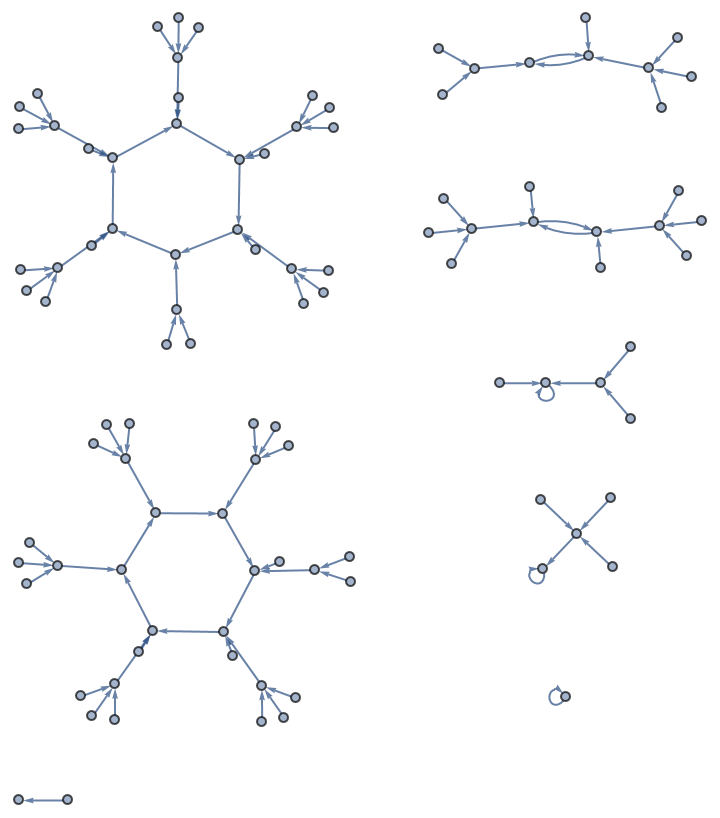
\includegraphics[scale=0.5]{DirectedGraphs.png}
\label{C1:Fig:Graphs}
\caption{Examples of graphs and their geometric realization.}
\end{figure}

Graphs have many applications due to their combinatorial construction. For example, we can consider the graph of all ``close'' words that start with ``dat'' in the English dictionary, with the derivation of the word as the relation for the edges (see Figure \ref{C1:Fig:Wordgraph}).

\begin{figure}[h]
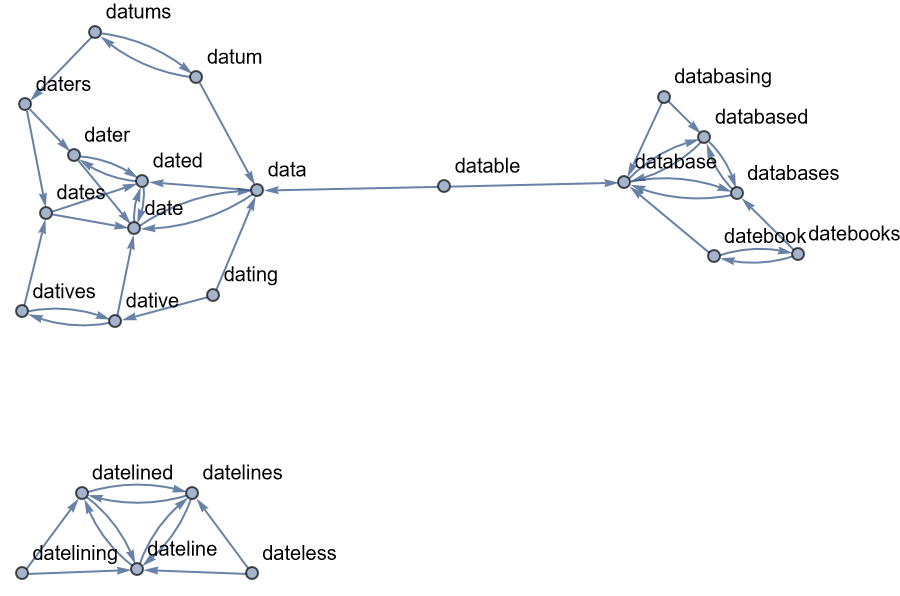
\includegraphics[scale=0.5]{Graph_Close_Words.png}
\label{C1:Fig:Wordgraph}
\caption{Graphs of close words with ``dat'' start.}
\end{figure}

For example, we can consider the graph $\Gamma$ given by $V=\{a,b,c,d\}$ and $E=\{(a,d),(b,d),(c,d)\}.$ Its geometric realization is a tripod in the plane. If we consider the collections
\begin{eqnarray*}
T_1 & =& \{\{(a,d)\},\{(b,d)\},\{(c,d)\}\} \\
T_2 & = &\{\{(a,d),a\},\{(b,d),b\},\{(c,d),c\},\{(a,d),(b,d),(c,d),d\}\}
\end{eqnarray*}
The collection $\tau=2^{T_1\cup T_2}$ is a topology for $\Gamma.$ Later we will see that this topology is related to the metric space structure on the graph.
\end{example}



\subsection{Exercises:}

\begin{enumerate}

\item Could the empty space be considered a topological space? In the case of a positive answer, describe a topology on it. 

\item Le $X=\{0,2,4,6,8\}$ and $\tau=\{\varnothing, \{0\},\{0,2\},\{0,4\},\{0,2,6\},\{0,4,6\},X\}.$ Is $\tau$ a topology for $X$? Elaborate your answer (this means you prove all topology properties or give a counter-example for those properties)

\item With the same $X$ as the previous exercise. Give a topology for $X$ with no open sets with two elements.

\item Prove that the discrete topology and the co-finite topology on $X$ are the same. 

\item Prove that if $X$ is any finite set, then the discrete topology and co-finite topology are the same. 

\item Give a counter-example of the previous statement when $X$ is an infinite set. \emph{Consider an ordered set of numbers.}

\item Given the graph $\Gamma=\left(\{a,b,c\},\{(a,b),(b,c),(c,a)\}\right).$ Find the sets $T_1$ and $T_2$ that \emph{generate} its topology.

\item Given a set $X,$ a \emph{basis} for a topology of $X$ is a collection $\mathcal{B}$ of subsets of $X$ (called base elements) such that:
\begin{itemize}
\item For each $x\in X,$ there is at least one base element $B$ containing $x.$
\item If $x$ belongs to the intersection of the base elements $B_1$ and $B_2,$ then there is a base element $B_3$ containing $x$ such that $B_3\subset B_1\cap B_2.$ 
\end{itemize}
If $\mathcal{B}$ satisfies both conditions, we define the \emph{topology generated by} $\mathcal{B}$ as: a subset $U$ of $X$ is said to be open in $X$ (an element of $\tau$) if for each $x\in U$ there is a base element $B\in\mathcal{B}$ such that $x\in B$ and $B\subset U.$

Using the previous definition, prove that the open intervals in $\mathbb{R}$ are a basis for a topology on it. This topology is called the standard topology on $\mathbb{R}.$ $\star$
\end{enumerate}

\section{Topological Properties}

In mathematics, each research field is conformed by a pair: the objects and the transformations, so we are interested in the properties of the objects that are preserved by the transformations. In the previous section, we introduce topological spaces, that correspond to the objects of topology. Lately, we will introduce the transformations, but now we will present a set of properties of topological spaces that will be of our interest during the study of data.


\subsection{Closedness}

We mentioned that topology is the study of spaces using a collection of subsets called: open sets. The first property is to complement the open sets. 

\begin{definition} 
Given a topological space $(X,\tau)$ and a subset $V$ of $X.$ We said that $V$ is closed if its complement in $X$ is an open set, i.e., $$X\setminus V:= \{x\in X: x\not\in V\}\in \tau.$$
\end{definition}

Closed sets on a topological space form a key part of topology, they are related to other topological properties and theorems. For example, closed sets are present in (topological) metric spaces to define continuity and compactness (we will see it later). Also, we can find closed sets in the definition of separation properties. 

\begin{example}
Assume that $X=\{1,3,5,7\}$ with the topology $\tau=\{\varnothing,\{1\},\{5\},\{1,5\},\{1,5,7\},X\}.$ 

In this topological space, the sets $\varnothing, \{1,\},\,\{3,7\},\{3,5,7\}, X,$ are closed sets. Even more, we can enumerate all closed sets of $X.$ 
\end{example}

Note that, in a topological space, some sets could have open and closed properties. In the previous example, $X$ is open and closed at the same time. In the literature, these sets are called \emph{clopen} sets, but on these notes, we will not give much attention to these.

\subsection{Connectedness}

As its name indicates, connectedness indicates if a set is made by a part or if it is a unit. Let me detail this. 

\begin{definition}
Given a set $V$ of a topological space, a partition of $V$ is a collection of open sets $\{A\}_j$ such that $A_i$
\end{definition}

\begin{definition}
Given a set $V$ of a topological space $X,$ we said that $V$ is \emph{not connected} if there exists open sets $A$ and $B,$ such that:
\begin{enumerate}
\item $V=A\cup B,$
\item $A\cap B =\varnothing.$
\end{enumerate}

On the contrary, if there is no such partition, then we say that $V$ is \emph{connected}
\end{definition}

\begin{example}
Assume that $X=\{1,3,5,7\}$ with the topology $\tau=\{\varnothing,\{1\},\{5\},\{1,5\},\{1,5,7\},X\}.$ 

The set $\{1,5\}$ is not connected, because $\{1,5\}=\{1\}\cup\{5\}.$ The sets $\{1\},\{5\},\{1,5,7\}, X$ are connected. 
\end{example}

\begin{example}
Assume that $X=\{1,3,5,7\}$ with the discrete topology $\tau=2^X.$ On this topology, $X$ is no longer connected, because: $$X=\{1\}\cup\{3,5,7\}=\{1,3\}\cup\{5,7\}.$$

In fact, the only connected sets are $\{1\},\{3\},\{5\}$ and $\{7\}.$
\end{example}

So connectedness of a space depends on the topology of the ambient space. 

\subsubsection{Connected compontents}

Between the connected subspaces of a topological space, some are characteristic of the space. Before we state the definition of connected components, we need to introduce the concept of equivalence relations.

In mathematics, we can relate objects by equivalence relations. In mathematics, a \emph{relation} between two sets $X$ and $Y$ is just a set of ordered pairs $(x,y),$ for example a function is a relation. The ``lower or equal'' ($\leq$) is a relation between real numbers.

\begin{definition}
An equivalence relation on a set $X,$ denoted by $\sim,$ is a mathematical relation that satisfies:
\begin{enumerate}
\item Reflexive: each element is related to itself $$a\sim a.$$

\item Symmetric: if $a$ is related to $b,$ then $b$ is related to $a.$ $$a\sim b\Rightarrow b\sim a.$$

\item Transitivity: if $a$ is related to $b,$ and $b$ is related to $c,$ then $a$ is related to $c.$ $$a\sim b \mbox{ and }b\sim c\Rightarrow a\sim c.$$
\end{enumerate}
\end{definition}

What does an equivalence relation imply on a set? Well, given an equivalence relation on a set, we can ``collect'' all interrelated elements in a subset of the ambient set. These collections of interrelated elements are called \emph{equivalence classes} and they produce a partition on the ambient set.

\begin{definition}
Let $X$ be a set with an equivalence relation $\sim.$ We define the equivalence class of $x$ as the set $$[x]:=\{y\in X: y\sim x\}.$$
Given the equivalence relation $[y],$ we say that $y$ is a class representative. 
\end{definition}
Examples of equivalence relations can be found in.
We will define an equivalence relation on topological spaces given by connected sets.
\begin{definition}
Let $(X,\tau)$ be a topological space. Let $\sim$ defined as follow, $x$ and $y$ are related ($x\sim y$) if and only if there exists a connected subspace of $X$ containing both points. 
The equivalence classes for this equivalence relation are called \emph{Connected components} of $X.$
\end{definition}
\begin{example}
Assume that $X=\{1,3,5,7\}$ with the topology $\tau=\{\varnothing,\{1\},\{5\},\{1,5\},\{1,5,7\},X\}.$ 

The unique connected component of $X$ is $X$ itself, and this follows because the space is connected on this topology.
\end{example}

\begin{example}
Assume that $X=\{1,3,5,7\}$ with the discrete topology $\tau=2^X.$ On this topology, $X$ is no longer connected, and the connected components are $\{1\},\{3\},\{5\}$ and $\{7\}.$
\end{example}

\subsubsection{Connectedness on Graphs}

As graphs are an essential part of TDA, we need to understand how it works connectedness over graphs. 

Let $\Gamma=(V, E)$ be a graph, and we will think that there is no distinction between the combinatorial object and the geometric realization. 

\begin{definition}
We say that $\Gamma$ is \emph{path-connected} if every two points can be joined by a trajectory of continuous edges. 
\end{definition}

\begin{proposition} 
Let $\Gamma=(V, E)$ be a path-connected graph, then $\Gamma$ is connected in the graph topology. 
\end{proposition}
\begin{proof}
Assume that $\Gamma$ is not path-connected. Then there exists at least a pair of points that are not connected by a path. 
\end{proof}

For graphs, the connected components look like subgraphs (subsets that are graphs) that are path-connected.

\begin{example}
Consider the graph $K_n$ given by $V=\{1,2,\cdots, n\}$ and $E=V\times V.$ By definition, this graph is path-connected for every $n.$ 
\end{example}

\begin{example}
Consider the graph given by $V=\{1,2,\cdots, n\}$ and $E$ given by these conditions:
\begin{itemize}
\item $(v,u)\in E$ if $u$ and $v$ are even.
\item $(v,u)\in E$ if $u$ and $v$ are odd.
\end{itemize}

By its definition, this graph is not path-connected and is composed of two connected components.
\end{example}

\subsection{Compactness}

As you can imagine, compactness observes if the set's elements are sort of close together.  


\begin{definition}
Let $(X,\tau)$ be a topological space and $E$ be a subset. An open cover for $E$ is a collection of open sets of $X,$ $\{U_\alpha\}_{\alpha\in A},$ such that $$E\subset \bigcup_{\alpha\in A} U_\alpha.$$
\end{definition}

\begin{definition}
For $(X,\tau)$ and $E$ be a subset. We said that $E$ is \emph{compact} if for every open covering for $E$, there exists a finite cover (finite number of elements) that covers $E.$
\end{definition}

\begin{example}
Consider the set of positive integers $X=\mathbb{N}$ with the discrete topology $\tau=2^{\mathbb{N}}.$ Every finite set is compact. 

Also, if $X$ has the co-finite topology, then also every finite set is compact.
\end{example}

Now, the compactness property seems artificial and that maybe all subsets are compact but this does not happen. In the next section, we will introduce more examples of all properties on metric spaces.

\subsection{Exercises:}

\begin{enumerate}

\item Let $X$ be a non-empty set with the discrete topology. Prove that for the topological space $(X,2^X),$ the only connected components of $X$ are singletons (sets with a unique element). $\star$

\item Is it true that for any non-empty set $X,$ with the trivial topology, is connected? Elaborate on your answer. 

\item Construct an example of a disconnected $X$ with only three connected components.

\item Construct an example of a graph with $n$ vertices that is connected but it is not the graph $K_n.$

\item Let $X=\mathbb{Z}$ give a topology on $X$ such that has two connected components. 

\item Is it true that for any non-empty set $X,$ with the trivial topology, is compact? Elaborate on your answer. 

\item Prove that $X=\mathbb{Z}$ with the discrete topology is not compact. (\emph{Hint: Try to construct an open covering on } $\mathbb{Z}$) $\star$
\end{enumerate}

\section{Metric Spaces and Metric Topology}

Metric spaces are an important set of examples for topology, this follows because their metric structure induces a natural topology on them.

\begin{definition}
Let $X$ be a non-empty set. A \emph{metric} on $X$ is defined as a function $d:X\times X\to \mathbb{R}$ that satisfies:
\begin{enumerate}
\item Non degeneracy: $d(p,q)=0$ if and only if $p=q.$
\item Symmetry: $d(p,q)=d(q,p).$
\item Triangle inequality: for every $p,q,r\in X,$ $$d(p,q)\leq d(p,r)+d(r,q).$$
\end{enumerate}

A \emph{metric space} is a pair $(X,d)$ where $d$ is a metric for $X.$
\end{definition}
\begin{example}
Let $X=\mathbb{R}$ and $d(x,y)=|x-y|,$ the function given by the absolute value. Then $(X,d)$ is a metric space. The metric $d$ is known as the standard metric on the set of real numbers.

We can consider the functions:
\begin{itemize}
\item $d_1(x,y)=\left|\ln\left(\frac{x}{y}\right)\right|.$

\item $d_2(x,y)=\frac{|x-y|}{1+|x-y|}.$
\end{itemize}

Both functions are metrics for $X.$
\end{example}

\begin{example}
Let $X=\mathbb{R}^n$ be the set of ordered $n-$tuples of real numbers. If $x=(x_1,\cdots,x_n)$ and $(y_1,\cdots,y_n),$ then let $$d(x,y)=\sqrt{\sum_{j=1}^n (x_j-y_j)^2}$$ this function makes $X$ a metric space, and it is known as the $\ell_2-$metric.

Similarly to the dimension one ($\mathbb{R}$), there are more than one metric on $\mathbb{R}^n,$ for example:

\begin{itemize}
\item The $\ell_\infty$ norm: $$d(x,y)=\max_{j=1,\cdots,n} \{|x_j-y_j|\}.$$

\item The $\ell_1$ norm: $$d(x,y)=\sum_{j=1}^n |x_j-y_j|.$$

\item The discrete metric: $$d(x,y)=1-\delta_{xy}.$$
\end{itemize}
\end{example}

The geometry of $\mathbb{R}^n$ changes for different metrics. For example, given a metric space $(X,d),$ a point $x\in X$ and a positive real number $r,$ we can define a special subset of $X,$ this subset is a \emph{ball} centered at $x$ of radius $r$:

$$B_d(x,r):=\left\{y\in X: d(x,y)< r \right\}.$$

You can look for example, at different balls plotted on each geometry in the next figure.

In the next example, we will assume that a graph $\Gamma$ means also its geometric representation in some $\mathbb{R}^n.$

\begin{example}
Given a graph $\Gamma=(V,E).$ We define the following metric on it. Let $d: V\times V \to \mathbb{R}$ given as follows: for any pair $(u,v),$ the number $d_\Gamma (u,v)$ is the length of the shortest path that joins $u$ and $v,$ and by length we mean the sum of the distance of between the points in a path for a given metric in $\mathbb{R}^n.$
\end{example}

In the literature, previous metrics on the graph can be uniformized by taking the distance between the vertices to be always one. 
\subsection{Metric Topology}

The metric space structure on a set $X$ induces a natural topology on it, this topology is known as the \emph{metric topology}. Before we state the description of open sets, we need to understand the concept of the basis for a topology.

\begin{definition}
Let $X$ be a set, a \emph{basis} for a topology on $X$ is a collection $\mathcal{B}$ of subsets of $X$ (called \emph{base elements}) that satisfies:
\begin{enumerate}
\item For each $x\in X,$ there is at least one base element of $B$ such that $x\in B.$
\item If $x$ belongs to the intersection of two base elements $B_1$ and $B_2,$ then there is a base element $B_3$ containing $x$ such that $$B_3\subset B_1\cap B_2.$$
\end{enumerate}

If $\mathcal{B}$ satisfies these two conditions, then we define the topology $\tau_{\mathcal{B}}$ generated by $\mathcal{B}$ as follows: A subset $U\subset X$ belongs to $\tau_{\mathcal{B}}$ if for each $x\in U$ there is a base element $B\in\mathcal{B}$ such that $x\in B\subset U.$
\end{definition}

The previous definition is nothing new, you have seen a similar concept in Complex Calculus when we talked about open subsets and neighborhoods of $\mathbb{C}.$

\begin{definition}
Let $(X,d)$ be a metric space. Consider the collection $\mathcal{B}_d$ as the set of all balls centered on points of $x$ of any radius. 

The topology on $X$ induced by the basis $\mathcal{B}_d$ is called the \emph{metric topology} on $X.$
\end{definition}

\begin{example}
Consider $\mathbb{R}^2$ with the euclidean metric (or standard metric), the basis of the topology $\mathcal{B}_d$ consists of all circular regions on $\mathbb{R}^2.$
\end{example}

The metric topology is very special because topological properties have a more detailed description here. In what follows, we will describe all topological properties for the metric topology. From now on, when we think of a metric space $(X,d)$ we will think $X$ endorsed with the induced metric topology.

\subsection{Closed sets}

\begin{definition}
Let $(X,d)$ be a metric space and $Q\in X$ a point set. We say that $q\in X$ is a \emph{limit point} (or \emph{accumulation point}) of $Q$ if for any real number $\varepsilon$ (no matter how small) there exists a point $p\in Q$ different from $q$ such that $$d(q,p)<\varepsilon.$$
\end{definition}

The previous definition, in topological terms, means that for a limit point $q,$ any ball centered at $q$ always intersects $Q$.

\begin{example}
Consider the set $(\mathbb{R},d)$ with the standard metric. The set $Q=\left\{\frac{1}{n}: n\in\mathbb{N}\right\},$ the point $0\in\mathbb{R}$ is a limit point for $Q.$ You can see in the next figure you can see a sketch of why.
\end{example}

\begin{example}
Consider the set $(\mathbb{R}^2,d)$ with the standard metric. The set $Q=\left\{\left(x,\frac{\sin(x)}{x}\right): x\in(0,\infty)\right\}.$ The point $(0,1)\in \mathbb{R}^2$ is a limit point for $Q.$
\end{example}

\begin{definition}
Let $(X,d)$ be a metric space and $Q\in X$ a point set. We call \emph{boundary} of $Q$ to the set of all its limit points, denoted by $\partial Q.$ The \emph{closure} of $Q$ is defined to be the union of $Q$ and its boundary, \emph{i.e.}, $$\overline{Q}=Q\cup \partial Q.$$ 

We say that $Q$ is closed in $X$ if it is equal to its closure: $$Q=\overline{Q}.$$
\end{definition}


\subsection{Compact Sets}

In the metric topology, compact sets have a more intuitive description. On metric spaces,  any compact set has to be closed and bounded, if one of these two properties fails the set cannot be compact. 

\begin{definition}
Let $Q$ be a subset of a metric space $(X,d).$ The diameter of $Q,$ denoted by $\mbox{\upshape{diam}}(Q),$ is the minimal possible upper-bound for all distances of points of $Q,$ \emph{i.e.}, $$\mbox{\upshape{diam}}(Q):=\sup_{x,y\in Q} d(x,y).$$ The diameter can be a real number or $\infty.$
\end{definition}


\begin{definition}
Let $Q$ be a subset of a metric space $(X,d).$ We say that $Q$ is \emph{bounded} if its diameter is finite. $$\mbox{\upshape{diam}}(Q)<\infty.$$
\end{definition}

\begin{example}
Let $(\mathbb{R},d)$ where $d$ is the euclidean metric. The set $Q=\left\{\frac{1}{n}: n\in\mathbb{N}\right\}$ is not compact. 

Note that even if the diameter of $Q$ is 1, the set is not closed because does not contain its limit point. 
\end{example}

\begin{proposition}
\label{C1:P1:CompactClosedBounded}
Let $X=\mathbb{R}^n$ and $d$ the standard metric. A subset $Q\subset \mathbb{R}^n$ is compact if and only if it is bounded and closed.
\end{proposition}

\begin{example}
Let $Q=\left\{\frac{1}{n}: n\in\mathbb{N}\right\}.$ In the previous example, we said that $Q$ is bounded but it is not closed. Therefore, from the previous proposition, $Q$ cannot be compact of $(\mathbb{R},d).$
\end{example}

Therefore, Proposition \ref{C1:P1:CompactClosedBounded} proposes a way to check if a set can be compact. For general metric spaces, the other direction of the proposition does not follow so easily, we need extra conditions on the metric space and these conditions are beyond the intentions of these notes. In the particular case of $\mathbb{R}^n$ with the euclidean metric, closed and bounded means compact.

\begin{theorem}
Let $Q\subset \mathbb{R}^n$ where $\mathbb{R}^n$ has the euclidean metric. Then $Q$ is compact if and only if it is closed and bounded.
\end{theorem}

The previous Theorem implies that whenever we look at a data set as a finite collection of points in some $\mathbb{R}^n,$ these sets are compact because they are bounded and closed.

You may ask, what happens with compactness in the case of metric graphs? Well, if the graph has finite vertices and its geometrization belongs to some $\mathbb{R}^n,$ then the graph is compact for the metric graph. But if the graph has infinite vertices, then this is another story, we need to be careful about how its metric is defined to determine if it is compact or not.

How we can infer the topological properties of a data universe via a data set? Well, a data set is a sample of a bigger space of information. If we look, for example, that in our sample (observations) there is some accumulation, then we can infer that close in that region we have accumulation points and the data universe could contain a closed subset which is not a finite set of points.

\subsection{Connected sets}

There is no particular change in the definition of connected sets in metric spaces, but limit points can be helpful when we look for a partition.

\begin{definition}
A point set $Q\in (X,d)$ is said to be disconnected if $Q$ admits a partition into two disjoint non-empty sets $U$ and $V$ so that there is no point in $U$ that is a limit point of $V$ and no point in $V$ that is a limit point of $U.$
\end{definition}

\begin{example}
The set $Q=\{\frac{1}{n}:n\in\mathbb{N}\}$ is disconnected in $(\mathbb{R},d).$
\end{example}

\begin{example}
The following sets are connected in $(\mathbb{R}^2,d):$

\begin{itemize}
\item A punctured ball centered at cero: $B_d(0,r)\setminus\{0\}.$

\item An anular region centered at cero: $B_d(0,r_1)\setminus B_d(0,r_2).$

\item An ball region without several regions removed:
\end{itemize}
\end{example}

\begin{theorem}
Let $(\mathbb{R},d)$ where $d$ is the euclidean metric. Then $[0,1]$ is compact and connected, and $(0,1)$ is connected.
\end{theorem}

\begin{proof}
That $[0,1]$ is compact follows from the fact that $[0,1]$ is closed and bounded. The prove that $[0,1]$ and $(0,1)$ are connected are similar. We will do it for $(0,1).$

Let 
\end{proof}

\subsection{Exercises:}

\begin{enumerate}

\item Prove that for $\mathbb{R}^3$ the following is a metric: $$d((x_1,x_2,x_3),(y_1,y_2,y_3))=\max |x_j-y_j|.$$ Also, provide a picture of a ball of radius $r$ centered at $(0,0,0).$

\item Let $(X,d)$ be any metric space. Prove that $$e(x,y)=\frac{d(x,y)}{1+d(x,y)}$$ is a metric for $X$ and $(X,e)$ has finite diameter. $\star$

\item Let $(X,d)$ where $X$ is any non-empty set and $d$ is the discrete metric (\emph{i.e.,} 1 if the points are different and 0 if they are the same). Prove that the metric topology of $(X,d)$ is the discrete topology (or equivalently, that any subset of $(X,d)$ is an open set).

\item Show that the open subsets of $\mathbb{R}\times\{0\}$ as subspace of $\mathbb{R}^2$ (with the standard topology) are of the form $U\times \{0\}$ where $U$ is open for $\mathbb{R}.$ Also, show that none of them are open sets of $\mathbb{R}^2.$

\item Find the interior and boundary of the following subsets of $\mathbb{R}^2.$
\begin{itemize}
\item $A=\{(x,y)\in\mathbb{R}^2: y=0\}.$
\item $B=\{(x,y)\in\mathbb{R}^2: x>0, y\neq 0\}.$
\item $C=\{(x,y)\in\mathbb{R}^2: 0<y^2-x^2<1\}.$
\end{itemize}

\item Determine the topological properties of the previous sets.

\item Consider the subset of $S\subset\mathbb{R}^2$ given by $$S:=\left\{\left(\frac{1}{n},\frac{1}{n}\right):n\in\mathbb{N}\right\}.$$ Compute $\overline{S}.$

\item Consider the set $E=([0,1]\times[-1,1]) \setminus \{(1/n,0): n\in\mathbb{N}\}.$ Is $E$ connected? $\star$

\end{enumerate}

\section{Special Subsets of $\mathbb{R}^n$}

In this section, we will present some special topological subspaces of $\mathbb{R}^n$ that will be of our interest during this course. 

\subsection{Balls and Spheres}

As in previous sections, we already stated the importance of balls in the topology of metric spaces, we will recall their definition and topological properties.

\begin{definition}
An \emph{euclidean ball} of radius $r>0$ and centered at $x_0$ in $\mathbb{R}^n$ is defined as the set $$\mathbb{B}^n:=\{x\in\mathbb{R}^n: d(x,x_0)<r\}.$$
\end{definition}

Balls are open and connected subspaces of $\mathbb{R}^n,$  but they are not compact. In the next Figure, we pictured balls of radius one centered at zero in dimensions: 1, 2, and 3.

\begin{definition}
An \emph{euclidean sphere} of radius $r$ and centered at $x_0$ in $\mathbb{R}^n$ is defined as the set $$\mathbb{S}^{n-1}:=\{x\in\mathbb{R}^n: d(x,x_0)=r\}.$$
\end{definition}

Spheres are closed, connected and compact subspaces of $\mathbb{R}^n.$ Even more, they coincide with the boundary of balls $\mathbb{B}^n.$ In the next Figure, we pictured balls of radius one centered at zero in dimensions: 1, 2, and 3.

\subsection{Simplices}

Simplices will be key for the Homology theory, so we will start our understanding of these subspaces.

\begin{definition}
A $n-$simplex in $\mathbb{R}^{n+1}$ is defined as the set $$K^n:=\{(x_1,x_2,\cdots, x_n,x_{n+1})\in \mathbb{R}^{n+1}: \sum_{j=1}^{n+1} x_j =1, x_j\geq 0\}.$$
\end{definition}

In the literature, you may find that simplices are defined as the convex hull of $(n+1)-$linear independent vectors in $\mathbb{R}^{n+1}$ (usually the standard basis of $\mathbb{R}^{n+1}$). Simplices are always connected, compact subspaces of $\mathbb{R}^{n+1}.$ 

\begin{example}
A $0-$simplex is just the point $x=1$ in $\mathbb{R}.$ A $1-$simplex is a segment of the line joining $(1,0)$ and $(0,1)$ in $\mathbb{R}^2.$ A $2-$simplex is the triangular region in $\mathbb{R}^2$ with vertices at $(0,0,1),\,(0,1,0)$ and $(1,0,0).$ A $3-$simplex is the region in $\mathbb{R}^4$ bounded by a tetrahedron with vertices at $(0,0,0,1),\,(0,0,1,0),\,(0,1,0,0)$ and $(1,0,0,0).$

In the next Figure, we pictured the first 4 simplices.
\end{example}

In general, a $n-$simplex contains all previous dimension simplices as boundaries. For example, a $2-$simplex has three $1-$simplices and $0-$simplices in its boundary. In the Chapter on Homology theory, we will see how the simplices relate to manifolds (topological subspaces) and what topological properties we can infer from this.



%\section{Special Metric Spaces}
%
%Of course, metric spaces theory is not only the study of $\mathbb{R}^n.$ In this section, we will provide a detailed introduction to other metric spaces that interest us.
%
%\subsection{Hamming Distance and Coding}
%
%
%\subsection{Intrinsic Metric}

\section{Homeomorphims}

Now that we have described the objects of Topology theory and their properties, we are interested in the set of transformations of topological spaces and how they interact with the topological properties.

In this section, we are interested in determining why a cube is ``topological equivalent'' to a sphere; intuitively, if our cube is made of a soft and malleable material, we can deform it into a sphere with ``continuous'' motions (no cuttings or gluing extra pieces). Therefore, for topologists studying the cube and the sphere represent the same, because their topologies are the same. 

How can we define this equivalence on topologies more formally? Well, we need to work to open sets and functions between spaces. Note that in the case of a cube in $\mathbb{R}^3$ for its (subspace) topology, the open sets look like disks, a bent disk or a cone-shaped disk, but at the end, if we flatten up all these open sets they look like disks. The open sets of a 2-sphere in $\mathbb{R}^3,$ for its (subspace) topology, look like curved disks and again if we flatten them up, they are just disks. Therefore, the topologies are the same. The function that makes the topological equivalence, is the composition of the two flattened-up processes. The functions that preserve open sets (send open sets to open sets) are called \emph{continuous} functions. 

\begin{definition}
A function $f$ between topological spaces $(X,\tau_X)$ and $(Y,\tau_Y)$ is said to be \emph{continuous} if for every open set $U\subset Y$ then $f^{-1}(U)$ is an open set in $(X,\tau_X).$
\end{definition}

In the literature, you may find that continuous functions between topological spaces are also called \emph{maps} or \emph{morphisms}. 

\begin{example}
Consider the topological spaces $(\mathbb{N},2^{\mathbb{N}})$ and $(2\mathbb{N},\tau)$ where $2\mathbb{N}$ is the set of even positive integers and $\tau$ is the trivial topology. Let $f:(\mathbb{N},2^{\mathbb{N}})\to (2\mathbb{N},\tau)$ given by $f(x)=2x.$

The function $f$ is continuous. Let see, for $(2\mathbb{N},\tau)$ there are only two open sets: $\varnothing$ and $2\mathbb{N}$ itself. 

First, $f^{-1}(\varnothing)=\varnothing$ since there is no element in $\varnothing,$ therefore $f^{-1}(\varnothing)$ is an open set in $(\mathbb{N},2^{\mathbb{N}}).$ For the case $f^{-1}(2\mathbb{N})$ note that for every element in $n\in 2\mathbb{N}$ we have that $\frac{n}{2}\in\mathbb{N}$.Therefore $f^{-1}(2\mathbb{N})=\mathbb{N}$ which is also an open set in $(\mathbb{N},2^{\mathbb{N}}).$

Therefore, the function $f(x)=2x$ is continuous in these topological spaces.
\end{example}

The continuity property of a function depends on the topologies of the domain and co-domain. For some topologies, a function could be continuous but if we change the topologies on these spaces the continuity fails.

\begin{example}
Consider again the function $f(x)=2x,$ but now between $(\mathbb{N},\tau)$ (with $\tau$ the trivial topology) and $(2\mathbb{N},2^{2\mathbb{N}}).$ For these topologies, the function $f$ is no longer continuous. Let $\{2,4\}\in 2^{2\mathbb{N}},$ this is an open set for $2\mathbb{N}$ and $f^{-1}(\{2,4\})=\{1,2\}$ which is not an open set in $(\mathbb{N},\tau).$ Since the continuity conditions fail for one open set, the function $f$ cannot be continuous.  
\end{example}

In order to give an equivalence relation between topological spaces we need that if $X$ is related to $Y,$ then $Y$ should be related to $X.$ The next definition, we will define the equivalence relation.

\begin{definition}
Let $(X,\tau_X)$ and $(Y,\tau_Y).$ An \emph{homeomorphism} is a bijective function $$h:(X,\tau_X)\to (Y,\tau_Y)$$ which is continuous and its inverse too.

If there exists a homeomorphism between $(X,\tau_X)$ and $(Y,\tau_Y),$ then we say that $(X,\tau_X)$ and $(Y,\tau_Y)$ are \emph{topological equivalent}.
\end{definition}

\begin{proposition}
Topological equivalence between topological spaces is an equivalence relation.
\end{proposition}
\begin{proof}
Note that for any topological space $(X,\tau),$ the identity map is continuous and its inverse is also the identity map. Therefore $(X,\tau)$ is topological equivalent to itself.

If $(X,\tau_X)$ is topological equivalent to $(Y,\tau_Y),$ then there exists a homeomorphism  $h:(X,\tau_X)\to (Y,\tau_Y).$ Note that if $h$ is a homeomorphism then $h^{-1}$ is it too. Therefore topological equivalence is symmetric.

If $(X,\tau_X)$ is topological equivalent to $(Y,\tau_Y),$ and $(Y,\tau_Y)$ to $(Z,\tau_Z).$ Then there are homeomorphisms $f$ and $g.$ Note that $g\circ f:(X,\tau_X)\to(Z,\tau_Z)$ is also a homeomorphism. Therefore, topological equivalence is transitive.
\end{proof}

\begin{example}
Consider the sets $\mathbb{N}$ and $2\mathbb{N}$ both the discrete topology. The map $f(n)=2n$ is a homeomorphism. Early, we saw that $f$ is continuous. 

Note that $f^{-1}(m)=\frac{m}{2}$ is also continuous.
\end{example}

\begin{example}
Consider $\mathbb{R}$ with the euclidean metric. Let $f:\mathbb{R}\to\mathbb{R}$ given by $$f(x)=3x+1.$$ From calculus, we know that $f$ is a continuous function (in the calculus sense but it coincides with the metric topology). For example, given a base element for the metric $(a,b),$ then $f\left((a,b)\right)=(3a+1,3b+1)$ this last one is also an open set of $\mathbb{R}.$

Note that $f^{-1}:\mathbb{R}\to\mathbb{R}$ is given by $f^{-1}(y)=\frac{y-1}{3}.$ $f^{-1}$ is also a continuous function, because $f^{-1}\left((a,b)\right)=\left(\frac{a-1}{3},\frac{b-1}{3}\right)$ which is an open set of $\mathbb{R}.$
\end{example}

\begin{example}
Let $\mathbb{R}$ with the euclidean metric and consider $(0,\infty)$ with the subspace topology of $\mathbb{R}.$ These two spaces are topological equivalent. Consider the function $f(x)=e^x.$ The function $f$ is bijective, for the following reasons:

\begin{itemize}
\item \textbf{Injective:} Let $x,y\in \mathbb{R}$ such that $f(x)=f(y),$ from the definition of $f$ we know that $f(x),f(y)\neq 0.$ Therefore $$\frac{f(x)}{f(y)}=e^{x-y}=1$$ and we know that the only solution to that equation is when $x-y=0,$ so $x$ should be equal to $y.$

\item \textbf{Surjective:} Let $y\in(0,\infty),$ and consider the number $x=\ln(y)\in\mathbb{R},$ from calculus we know that $$f(x)=e^{\ln(y)}=y.$$ Therefore, $f$ is surjective.  
\end{itemize}

The function $f$ is continuous, because $f\left((a,b)\right)$ is $(e^a,e^b)$ which is an open set for $(0,\infty)$ in the subspace topology.
\end{example}

\begin{example}
\label{C1:S6:ExampleInversion}
Consider $\mathbb{R}^2$ with the euclidean metric. Let $X=\mathbb{R}^2\setminus B((0,0),1)$ and $Y=B((0,0),1)\setminus\{(0,0)\}$ with the subspace topology. These spaces are topological equivalents. Consider the function 

\begin{eqnarray*}
f(x):&B((0,0),1)\setminus\{(0,0)\}\to \mathbb{R}^2\setminus B((0,0),1)\\
 &(x,y)\mapsto \left(\frac{x}{x^2+y^2},\frac{y}{x^2+y^2}\right)
\end{eqnarray*}

It is not difficult to prove that the image of any circle is again a circle, therefore for each base element of the subspace topology in $Y$ we have that its image is again a base element in $X$ for the subspace topology.

To see that the function is bijective it suffices to check that every circle of radius $0<r<1$ centered at $(0,0)$ is mapped to a circle with radius $>1$ bijectively. 

We know that every circle centered at $(0,0)$ is parametrized by $$(r\cos\theta,r\sin\theta)\quad \theta\in[0,2\pi)$$ and this parametrization is a bijective map from $[0,2\pi)$ to the circle. Note that $$f\left(r\cos\theta,r\sin\theta\right)=\left(\frac{\cos\theta}{r},\frac{\sin\theta}{r}\right).$$ If $0<r<1,$ then $\frac{1}{r}>1.$ So each circle in $Y$ is mapped to a unique circle in $X.$ The bijective property on $f$ follows from functions properties.
\end{example}

Finding homeomorphisms between topological spaces is not always possible, but there is a property on continuous functions that allow us to ``approximate'' homeomorphisms.

\begin{definition}[Embedding]
A function $g:(X,\tau_X)\to (Y,\tau_Y)$ is said to be an \emph{embedding} if it is a continuous injective function.
\end{definition}

Embeddings allow us to determine when a topological space can be seen as a subspace of another topological space. In particular, embeddings transform into homeomorphisms when we restrict the function to their image (the topological subspace with the subspace topology).

\begin{example}
\label{C1:S6:Example:Circleembedding}
In example \ref{C1:S6:ExampleInversion}, we mentionned the function 
\begin{eqnarray*}
f(x):&[0,2\pi)\to \mathbb{R}^2\\
 &\theta \mapsto \left(\cos\theta,\sin\theta\right).
\end{eqnarray*}

This function is an embedding of $[0,2\pi)$ into $\mathbb{R}^2.$ We already know that this function is continuous and the injective part follows from the fact that functions $\cos$ and $\sin$ are injective on $[0,2\pi).$
\end{example}


Finding homeomorphisms between general topological spaces is quite hard, therefore how do we determine when two topological spaces are equivalent? Well, topological properties (closedness, connectedness, and compactness) help us in this case, it turns out that these topological properties are preserved by homeomorphisms. Checking if the topological spaces present the same properties then it is possible that they are equivalent, but if don't then we know for sure that they are not equivalent. 

\begin{theorem}
\label{C1:S6:Theorem:Connected}
The image of a connected space under a continuous map is connected.
\end{theorem}
\begin{proof}
Let $f: X\to Y$ be a continuous map and let $X$ be connected. We wish to prove that the image $Z=f(X)$ is connected. From the fact that $f$ restricted to its image is also continuous, it suffices to prove it for surjective continuous functions $$g: X \to Z.$$ Suppose that $Z=A\cup B$ is a separation for $Z$ into two disjoint nonempty open sets in $Z.$ Since $g$ is continuous, $g^{-1}(A)$ an d$g^{-1}(B)$ are open sets whose union is $X.$ We know that both inverse images are disjoint because $g$ is surjective. Therefore $$X=g^{-1}(A)\cup g^{-1}(B)$$ is a separation for $X.$ Since $X$ is connected, one of the sets is empty, and so it is its image. Therefore $Z$ is connected. 
\end{proof}

\begin{example}
The previous theorem allows us to easily determine that  $\mathbb{R}$ (with the euclidean metric topology) and  $\mathbb{R}\setminus\{0\}$ (with the subspace topology) are not topologically equivalent. This follows from the fact that $\mathbb{R}\setminus\{0\}$ is not connected, actually $$\mathbb{R}\setminus\{0\}=(-\infty,0)\cup(0,\infty).$$ However, $\mathbb{R}$ is connected.
\end{example}

\begin{example}
The embedding from $[0,2\pi)$ to $\mathbb{R}^2$ in \ref{C1:S6:Example:Circleembedding}, implies that the circle is connected for the subspace topology. 
\end{example}

As we mentioned before, Theorem \ref{C1:S6:Theorem:Connected} is not enough to determine if two subspaces are or are not equivalent. Consider the following counterexample. 

\begin{example}
Consider the space $\mathbb{R}^2$ with the euclidean metric topology, and $\mathbb{R}^2\setminus\{(0,0)\}$ with the subspace topology. Both spaces are connected, but they are not topologically equivalent. The inequivalence follows from the existence of the puncture in $\mathbb{R}^2\setminus\{0\}.$ In subsequent chapters, we will introduce the Homotopy theory and we will be able to prove this inequivalence.
\end{example}

\begin{theorem}
The image of a compact space under a continuous map is compact.
\end{theorem}
\begin{proof}
Let $f:X \to Y$ be a continuous function and let $X$ be a compact topological space. Let $\mathcal{A}$ be a covering set for $f(X)$ by open subsets of $Y.$ By continuity, $$\left\{f^{-1}(A):A\in\mathcal{A}\right\}$$ is a open cover for $X.$ Since $X$ is compact (by hypothesis), there exist finitely many open sets that cover $X,$ let's say $$f^{-1}(A_1),\hdots, f^{-1}(A_n).$$ Then the sets $A_1,\hdots, A_n$ cover $f(X).$

Since our election of covering was arbitrary, we can say that $f(X)$ is compact.
\end{proof}

\begin{example}
The previous theorem allows us to easily determine that  $[0,1]$ and  $(0,1),$ as topological subspaces of $\mathbb{R},$ are not topologically equivalent. This follows from the fact that $[0,1]$ is compact but $(0,1)$ is not. 

In general, the open balls in $\mathbb{R}^n$  (with the euclidean metric) are not topologically equivalent to its closure. 
\end{example}


Compactness is not a sufficient condition to determine topological equivalence. The next counterexample.

\begin{example}
Consider the subspaces $\mathbb{S}^1$  and $\mathbb{S}^2$ both embedded in $\mathbb{R}^3$ with the subspace topology. Both subspaces are compact but they are not topologically equivalent. Again, this follows from the Homotopy theory.
\end{example}

We first ask why a donut and a mug are the same under topological eyes. Well, this follows from the fact that they are topologically equivalent but it is not easy to find the homeomorphism. How we can assure that those spaces are equivalent if we cannot construct a homeomorphism? With help of an \emph{isotopy}, we can prove the answer to the first question.

\begin{definition}
Let $X,Y\subset \mathbb{R}^n$ two subspaces. An \emph{isotopy} is a continuous map $$\xi: X\times [0,1] \to \mathbb{R}^n$$ such that: 
\begin{enumerate}
\item $\xi(X,0)=X,$
\item $\xi(X,1)=Y,$
\item and for every $t\in[0,1],$ $\xi(\cdot,t)$ is an homeomorphism between $X$ and the image of $\xi(\cdot,t).$ 
\end{enumerate}
\end{definition}

Isotopies are continuous deformations of one space into another, but there are some restrictions on these deformations: we cannot self-intersect the space during the deformation, and we cannot break into pieces something that is connected.

Using the isotopy construction, we can deform a mug into a donut without a problem, and since every step ($t\in [0,1]$) of the isotopy function is a homeomorphism, we have that both spaces are topologically equivalent. 

Some spaces are topologically equivalent but they are not isotopic (there is no isotopy between them), look at the following example.

\begin{example}
A mathematical knot is an embedding of $\mathbb{S}^1$ into $\mathbb{R}^3 or \mathbb{S}^3.$ From its definition, a knot is topologically equivalent to $\mathbb{S}^1.$ Nevertheless, they are not isotopic because if we want to ``unknot'' the knot we are forced to self-intersect the circle.

\begin{figure}[h]
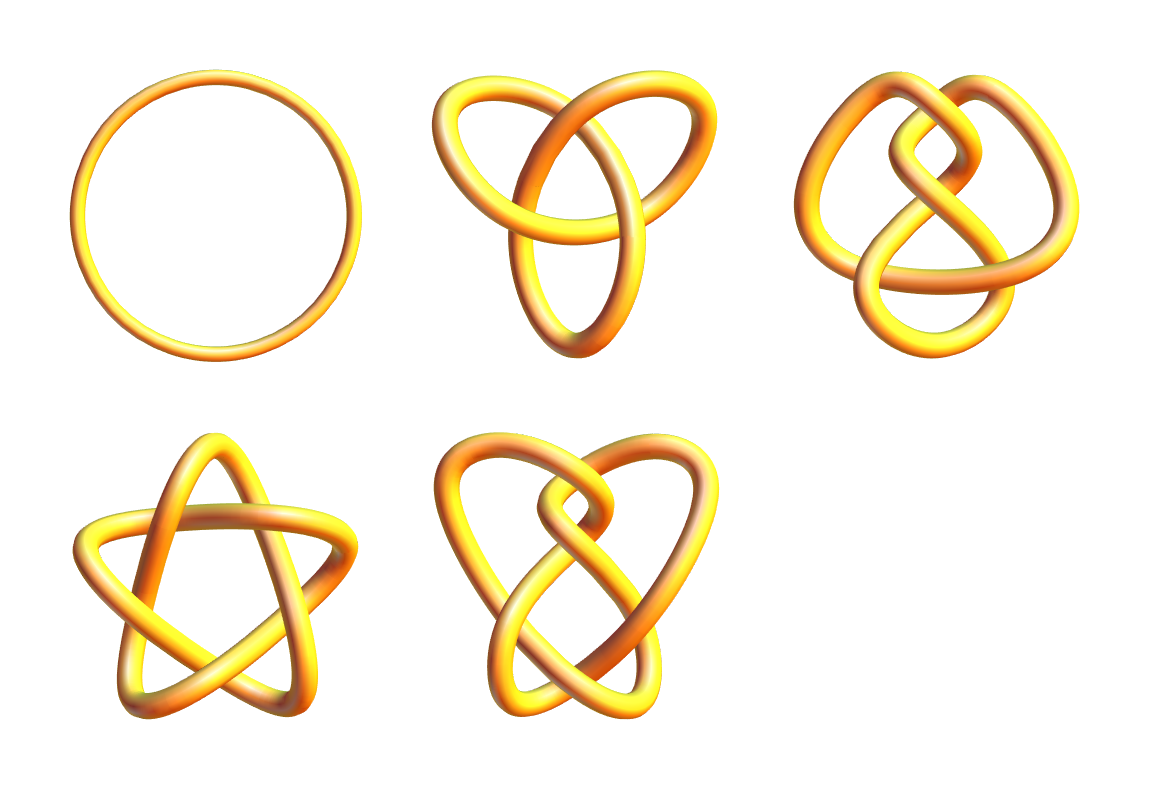
\includegraphics[scale=0.5]{O_168.png}
\caption{Examples of knots in $\mathbb{R}^3.$}
\end{figure}
\end{example}

\subsection{Exercises:}

\begin{enumerate}

\item Using continuous functions, what you can say about the topological properties of the following spaces?
\begin{itemize}
\item $A=\left\{(x,y)\in\mathbb{R}^2: xy=1\right\}.$
\item $A=\left\{(x,y,z)\in\mathbb{R}^2: 2z^2+3y^2+x^2=1\right\}.$
\end{itemize}

\item Prove that if $f:X\to Y$ is a continuous map, and $X$ is path-connected. Then $Y$ is path-connected too.

\item Show that the square $[0,1]\times[0,1]\in \mathbb{R}\times\mathbb{R}$ is homeomorphic to the torus.

\begin{figure}[h]
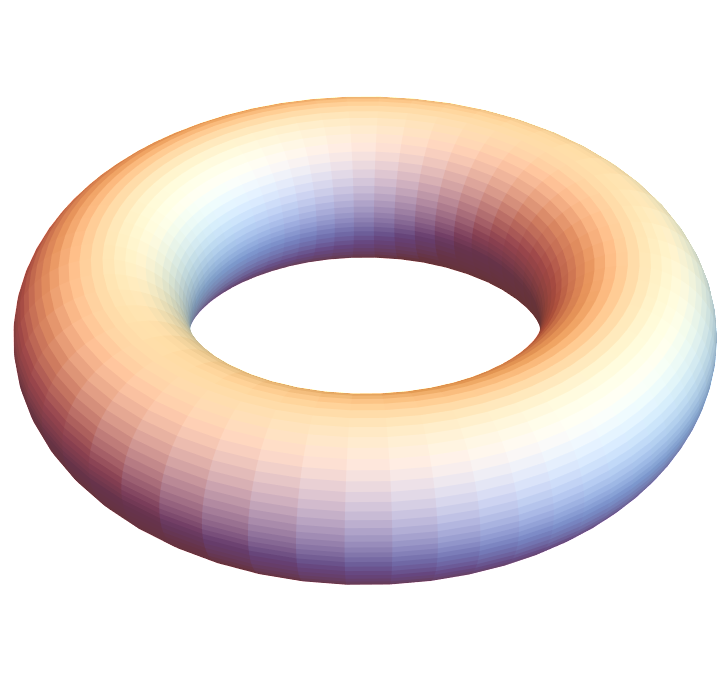
\includegraphics[scale=0.1]{Torus.png}
\caption{Torus surface in $\mathbb{R}^3.$}
\end{figure}


\item Find an isotopy between $X=\{(x,\sin(x)): x\in[0,2\pi]\}$ and $Y=\{(x,\cos(x)):x\in[0,2\pi]\}$ spaces of $\mathbb{R}^2.$

\item Show that $f:\mathbb{R}\to \mathbb{R}^2$ given by $f(x)=(x,\cos(x))$ is an embedding.

\item What can you say about the subspace $S=\left\{(x,x\sin\left(\frac{1}{x}\right): x\in (0,1]\right\}\cup\{(0,0)\}.$

\item Suppose that $f:X\to Y$ is continuous. If $x\in X$ is a limit point for some subset $A\subset X.$ Is it necessarily true that $f(x)$ is a limit point of $f(A)$? $\star$

\item Show that the subespace $(a,b)\subset \mathbb{R}$ is homeomorphic to $(0,1).$

\item Let $f:A\to B$ and $g:C\to D$ two continuous functions. Let us define the map $f\times g:A\times C \to B\times D$ by the equation $$(f\times g)(a\times c)=f(a)\times g(c).$$ Show that $f\times g$ is continuous. (\textit{Hint: Do research about product spaces and product topology}) $\star$

\item Let $X$ be a metric space with metric $d.$ Show that $d:X\times X\to \mathbb{R}$ is continuous.

\item Let $(X,d_X)$ and $(Y,d_Y)$ be two metric spaces. Let $f:X\to Y$ that satisfies $$d_Y(f(x_1),f(x_2))=d_X(x_1,x_2).$$ Show that $f$ is an embedding. 

\item Show that $\mathbb{R}^n$ and $\mathbb{R}$ are not homeomorphic for $n>1.$ $\star$

\end{enumerate}

\section{Quotient spaces and their topology}

Unlike previous constructions, Quotient topology is not a natural generalization of something that you already studied in calculus or analysis. Nevertheless, its fundaments come from geometry where we can ``cut-and-paste'' pieces to obtain something new. 

A cylinder is a naive example, if we take a rectangle in $\mathbb{R}^2$ we can use a map (continuous function) that sends one of the big sides into the other and we can ``glue them''.  If we extend this example, and ``glue'' the end circles of the triangle, we obtain a surface torus. Some of you may be familiar with the schema presented in Figure \ref{Fig:TorusDiag}.

 \begin{figure}[h]
 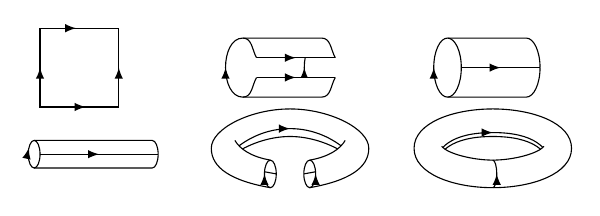
\begin{tikzpicture}[scale=0.5]
  % lattice
%  \draw[->,ultra thick] (-2,0) -- (2,0);
%  \draw[->,ultra thick] (0,-2) -- (0,2);
%  \draw (-2,-2) grid (2,2);
%  \node [draw,ultra thick,rectangle,minimum width=1cm,minimum height=1cm,label=below:$2 \pi$,label=right:$2 \pi$] at (0.5,0.5) {};

  % square
  \begin{scope}[xshift=4cm,yshift=1cm]
    \draw[postaction={decorate},decoration={
          markings,
          mark=at position .145 with {\arrow{latex}},
          mark=at position .375 with {\arrow{latex}},
          mark=at position .635 with {\arrowreversed{latex}},
          mark=at position .875 with {\arrowreversed{latex}},
        }
    ]
    (0,-1) -- +(2,0) -- +(2,2) -- +(0,2) -- cycle;
  \end{scope}

  % bracelet
  \begin{scope}[xshift=9.5cm,yshift=1cm]
    \draw[postaction={decorate},decoration={
          markings,
          mark=at position .5 with {\arrow{latex}}
        }
    ]
    (0,.25) -- ++(2,0);
    \draw[postaction={decorate},decoration={
          markings,
          mark=at position .5 with {\arrow{latex}}
        }
    ]
    (0,-.25) -- ++(2,0);
    \draw[postaction={decorate},decoration={
          markings,
          mark=at position .5 with {\arrow{latex}},
        }
    ] (0,-.25) to[out=-120,in=0] (-.35,-.75) to[out=180,in=180] (-.35,.75) to[out=0,in=120] (0,.25);
    \draw (2,.25) to[out=120,in=0] (1.65,.75) -- (-.35,.75) (-.35,-.75) -- (1.65,-.75) to[out=0,in=-120] (2,-.25);
    \begin{scope}
      \clip (0,.25) rectangle (2,-.25);
      \draw[postaction={decorate},decoration={
            markings,
            mark=at position .5 with {\arrowreversed{latex}},
          }
      ] (1.65,.75) to[out=180,in=180] (1.65,-.75);
    \end{scope}
  \end{scope}

  % cylinder
  \begin{scope}[xshift=14.7cm,yshift=1cm]
    \draw[postaction={decorate},decoration={
          markings,
          mark=at position .5 with {\arrow{latex}},
        }
    ] (0,0) -- (2,0);
    \draw[postaction={decorate},decoration={
          markings,
          mark=at position .5 with {\arrow{latex}},
        }
    ] (0,0) arc[start angle=0,delta angle=-360,x radius=.35,y radius=.75];
    \draw (2,0) arc[start angle=0,delta angle=-90,x radius=.35,y radius=.75] -- ++(-2,0);
    \draw (2,0) arc[start angle=0,delta angle=90,x radius=.35,y radius=.75] -- ++(-2,0);
  \end{scope}

  % long cylinder
  \begin{scope}[xshift=4cm,yshift=-1.2cm]
    \draw[postaction={decorate},decoration={
          markings,
          mark=at position .5 with {\arrow{latex}},
        }
    ] (0,0) -- (3,0);
    \draw[postaction={decorate},decoration={
          markings,
          mark=at position .6 with {\arrow{latex}},
        }
    ] (0,0) arc[start angle=0,delta angle=-360,x radius=.15,y radius=.35];
    \draw (3,0) arc[start angle=0,delta angle=-90,x radius=.15,y radius=.35] -- ++(-3,0);
    \draw (3,0) arc[start angle=0,delta angle=90,x radius=.15,y radius=.35] -- ++(-3,0);
  \end{scope}

  % open torus
  \begin{scope}[xshift=9cm,yshift=-1.7cm]
    \draw[postaction={decorate},decoration={
          markings,
          mark=at position .5 with {\arrow{latex}},
        }
    ] (1,0) arc[start angle=0,delta angle=-360,x radius=.15,y radius=.35];
    \draw (1,0) ++(-.15,-.35) .. controls +(170:1) and +(-90:.5) .. ++(-1.5,1) .. controls +(90:.5) and +(180:1) .. ++(2,1) .. controls +(0:1) and +(90:.5) .. ++(2,-1) .. controls +(-90:.5) and +(10:1) .. ++(-1.5,-1) coordinate (a);
    \draw[postaction={decorate},decoration={
          markings,
          mark=at position .5 with {\arrow{latex}},
        }
    ] (a) ++(-.15,.35) arc[start angle=0,delta angle=-360,x radius=-.15,y radius=.35];
    \draw (1,0) ++(-.15,.35) .. controls +(170:.5) and +(-60:.25) .. ++(-.9,.5) coordinate (b);
    \draw (a) ++(0,.7) .. controls +(10:.5) and +(240:.25) .. ++(.9,.5) coordinate (c);
    \begin{scope}
      \clip (1,0) ++(-.15,.35) .. controls +(170:.5) and +(-60:.25) .. ++(-.9,.5) -- ++(0,2) -| (c) .. controls +(240:.25) and +(10:.5) .. ++(-.9,-.5);
      \draw (1,0) ++(-.15,-.35) ++(0,-.7) .. controls +(170:1) and +(-90:.5) .. ++(-1.5,.8) .. controls +(90:.5) and +(180:1) .. ++(2,1.2) .. controls +(0:1) and +(90:.5) .. ++(2,-1.2) .. controls +(-90:.5) and +(10:1) .. ++(-1.5,-.8);
      \draw[postaction={decorate},decoration={
            markings,
            mark=at position .5 with {\arrow{latex}},
          }
      ] (1,0) ++(-.15,-.35) ++(0,-.8) .. controls +(170:1) and +(-90:.5) .. ++(-1.5,.8) .. controls +(90:.5) and +(180:1.2) .. ++(2,1.5) .. controls +(0:1.2) and +(90:.5) .. ++(2,-1.5) .. controls +(-90:.5) and +(10:1) .. ++(-1.5,-.8);
    \end{scope}
    \begin{scope}
      \clip (a) ++(-.15,.35) arc[start angle=0,delta angle=-360,x radius=-.15,y radius=.35];
      \draw (a) ++(-.15,.35) .. controls +(10:1) and +(-90:.5) .. ++(1.5,.8);
    \end{scope}
    \begin{scope}
      \clip (1,0) arc[start angle=0,delta angle=-360,x radius=.15,y radius=.35];
      \draw (1,0) .. controls +(170:1) and +(-90:.5) .. ++(-1.5,.8);
    \end{scope}
  \end{scope}

  % torus
  \begin{scope}[xshift=14cm,yshift=-1.7cm]
    \draw[postaction={decorate},decoration={
          markings,
          mark=at position .5 with {\arrowreversed{latex}},
        }
    ] (1.5,.35) arc[start angle=90,end angle=-90,y radius=.35,x radius=.1];
    \draw (1.5,-.35) .. controls +(180:1) and +(-90:.65) .. ++(-2,1) .. controls +(90:.65) and +(180:1) .. ++(2,1) .. controls +(0:1) and +(90:.65) .. ++(2,-1) .. controls +(-90:.65) and +(0:1) .. ++(-2,-1); \draw (1.5,.35) .. controls +(180:.5) and +(-50:.25) .. ++(-1.3,.35) coordinate (b);
    \draw (1.5,.35) .. controls +(0:.5) and +(230:.25) .. ++(1.3,.35) coordinate (c);
    \begin{scope}
      \clip (1.5,.35) .. controls +(180:.5) and +(-50:.25) .. ++(-1.3,.35) -- ++(0,2) -| (c) .. controls +(230:.25) and +(0:.5) .. ++(-1.3,-.35);
      \draw (1.5,-.35) ++(0,-.7) .. controls +(180:1) and +(-90:.65) .. ++(-1.5,1) .. controls +(90:.65) and +(180:1) .. ++(1.5,1) .. controls +(0:1) and +(90:.65) .. ++(1.5,-1) .. controls +(-90:.65) and +(0:1) .. ++(-1.5,-1);
      \draw[postaction={decorate},decoration={
            markings,
            mark=at position .5 with {\arrow{latex}},
          }
      ] (1.5,-.35) ++(0,-.6) .. controls +(180:1) and +(-90:.65) .. ++(-1.5,1) .. controls +(90:.65) and +(180:1) .. ++(1.5,1) .. controls +(0:1) and +(90:.65) .. ++(1.5,-1) .. controls +(-90:.65) and +(0:1) .. ++(-1.5,-1);
    \end{scope}
  \end{scope}

\end{tikzpicture}
\label{Fig:TorusDiag}
\caption{Torus gluing diagram from a rectangle.}
 \end{figure}
 
 This ``gluing'' process allows us to create new topological spaces. In this section, we will introduce what we understand by ``gluing'' in a formal way and how to describe the topology of these ``glued'' spaces.
 
 Before defining a quotient space, recall the definition of equivalence relation introduced in Section.
 
 \begin{definition}
 Let $(X,\tau_X)$ be a topological space, and let $\sim$ be an equivalence relation on $X.$ The \emph{quotient set} is defined as the set $$Y=X/_\sim=\{[x]: x\in X\}$$ where $[\cdot]$ denotes the equivalence classes of $X$ under $\sim.$
 \end{definition}
 
The previous definition just says that a quotient space is a set consisting of all existing different equivalence classes on $X.$ 

\begin{example}
Let $(\mathbb{N},2^{\mathbb{N}})$ with the equivalence relation $x\sim y$ if and only if 2 divides $x$ and $y,$ or none of them.

The quotient space is just the set $\{[1],[2]\}.$
\end{example}

\begin{example}
Let $[0,1]\times[0,1]$ with the subspace topology of $\mathbb{R}^2.$ Consider the equivalence relation: $(x_1,y_1)\sim (x_2,y_2)$ if and only if one these are true
\begin{itemize}
\item $x_1=x_2,$  $y_i=0$ and $y_j=1.$
\item $y_1=y_2,$ $x_i=0$ and $y_j=1.$
\end{itemize}

There are four types of equivalence classes: 
\begin{itemize}
\item $[(0,0)]=\{(0,0),(0,1), (1,1),(1,0)\},$
\item $[(x,0)]=\{(x,0),(x,1)\}$ with $x\in(0,1).$
\item $[(0,y)]=\{(0,y),(1,y)\}$ with $y\in (0,1).$
\item $[(x,y)]=\{(x,y)\}$ with $(x,y)\in(0,1)\times(0,1).$
\end{itemize}
\end{example}
 
 What can you say about the last example? It looks familiar, well the quotient space is the torus surface. 
 
 \begin{definition}
 Let $(X,\tau_X)$ be a topological space and $Y=X/_\sim$ be a quotient space. The \emph{quotient topology} on $Y$ is defined as follows: $U\subset Y$ is an open set if and only if $$\{x\in X:[x]\in U\}\in \tau_X.$$
 
 The quotient set with the quotient topology is known as a \emph{quotient space}.
 \end{definition}
 
 \begin{example}
 For our first example $Y_1=\mathbb{N}/_\sim,$ the quotient topology coincides with the discrete topology on a space of two elements. Note that $\{[1]\}$ is open, because $\{1,3,5,7,9,\cdots\}$ is a open subset for $\mathbb{N}.$ For similar reason, $\{[2]\}$ is also open.
 \end{example}
 
 \begin{example}
 For our second example $Y_2={}^{[0,1]\times[0,1]}/_\sim,$ the quotient space have three types of opens sets:
 \begin{itemize}
 \item The neighborhoods of $[(0,0)],$ these open sets are like a circle formed by 4 pieces (each with their center in the corners of the rectangle).
 
 \item The neighborhoods of $[(x,0)]$ or $[(0,y)],$ these open sets are like a circle formed by 2 pieces (cut over a diameter).
 
 \item The neighborhoods of $[(x,y)]$ that are usual disks.
 \end{itemize}
 \end{example}
 
\begin{definition}
Let $(X,\tau_X)$ and $X/_\sim$ a quotient space. Let $\pi: X\to X/_\sim$ be the function that sends each element to its equivalence class, \emph{i.e.}, $$x\mapsto [x].$$

This function $\pi$ is called the \emph{canonical projection} and it is an embedding.
\end{definition}

\subsection{Crushing things}

Let $(X,\tau_X)$ be a topological space, and $A\subset X$ be a set. Let $\sim$ the equivalence relation on $X$ given by $x\sim y$ if and only if $x,y\in A.$ The last equivalence relation, breaks $X$ into two different types of classes: $A$ and $\{x\}.$  In the quotient space $X/\sim,$ the set $A$ is ``crushed'' into a point, and the original topological space ``deforms'' from its original form; from this fact, we will denote $X/\sim$ by $X/A.$

\begin{example}
Let $X=[0,1]$ with the subspace topology and $A=\partial X=\{0,1\}.$ The quotient space $X/A$ is homeomorphic to $\mathbb{S}^1.$

This homeomorphism is because $(0,1)$ remains the same, and $0$ and $1$ are identified into a single point.
\end{example}

\begin{example}
Let $X=\overline{B((0,0),1)}$ the closed disk in $\mathbb{R}^2$ with the subspace topology, and let $A=\partial X.$ Then $X/A$ is homeomorphic to $\mathbb{S}^2$ with the subspace topology.
\end{example}

\begin{example}
Let $X$ be the surface torus, and $A$ be one of its meridians. Then $X/A$ is called a \emph{pinched torus}.
\end{example}


\subsection{Quotients and continuous functions}

One could ask, what happens to a continuous function $f: X\to Y$ if we define a quotient space from $X$? Does the continuity follow being true for the new function? Well, the answer is \textit{depends} on the definition of the function $f$ and the equivalence relation.

\begin{definition}
Let $f: X\to Y$ be a continuous function and let $\sim$ be an equivalence relation on $X.$ We way that $f$ \emph{descends} to the quotient if there exists a continuous function $$\hat{f}:{}^X/_\sim \to Y$$ such that $\hat{f}=f\circ \pi,$ where $\pi: X\to {}^X/_\sim.$ The function $\hat{f}$ is also continuous.
\end{definition} 


\begin{example}
Let $(\mathbb{N},2^{\mathbb{N}})$ with the equivalence relation $x\sim y$ if and only if 2 divides $x$ and $y,$ or none of them.

The quotient space is just the set ${}^{\mathbb{N}}/_\sim=\{[1],[2]\}.$ Let $Y=\{0,1\},$ with the discrete topology and define the map

\begin{eqnarray*}
f: & \mathbb{N} \to Y \\
& x\mapsto x\pmod 2
\end{eqnarray*} where $x\pmod 2$ is just the reminder of the division of $x$ by two. The function $f$ descends to the quotient.
\end{example}

\begin{example}
Let $X=[0,1]\times\{0\}$ with the subspace topology of $\mathbb{R}^2,$ and consider the quotient space $X/A$ where $A=\partial X.$ The function $f:[0,1]\times\{0\} \to \mathbb{R}^2$ given by $$f(x,0)=\left(\frac{1}{2}-x^3,0\right)$$ descends to the quotient. 

figura ejemplo 
\end{example}

\section{Exercises}

\begin{enumerate}
\item Let $\mathbb{R}^2$ with the standard topology. Consider the following relation on $\mathbb{R}^2:$ $(x_1,y_1)\sim (x_2,y_2)$ if and only if $(x_1-x_2,y_1-y_2)\in\mathbb{Z}^2.$
\begin{enumerate}
\item Prove that $\sim$ is an equivalence relation in $\mathbb{R}^2.$
\item Describe the set of equivalence classes.
\item In case that $\sim$ is an equivalence relation, describe the open sets for ${}^{\mathbb{R}^2}\!/_\sim$.
\item Do you know a topological space that could be homeomorphic to ${}^{\mathbb{R}^2}\!/_\sim$
\end{enumerate}

\item  Let $\mathbb{S}^1$ embedded in $\mathbb{C}^1$ as the set of $\{z\in\mathbb{C}: z=e^{i\pi\theta},\theta\in\mathbb{R}\}$ and $\mathbb{C}^1$ with the metric topology. Consider the following relation on $\mathbb{S}^1:$ $z_1\sim z_2$ if and only if $\arg(z_1)-\arg(z_2)\in\mathbb{Z}.$
\begin{enumerate}
\item Prove that $\sim$ is an equivalence relation in $\mathbb{S}^1.$
\item Describe the set of equivalence classes.
\item Do you know a topological space that could be homeomorphic to ${}^{\mathbb{S}^1}\!/_\sim$
\end{enumerate}

\item Let $X=\mathbb{R}^2\setminus\{(0,0)\}$ with the subspace topology. Consider the following relation on $\mathbb{R}^2\setminus\{(0,0)\}$: $(x_1,x_2)\sim (y_1,y_2)$ if and only if there exists $c\in\mathbb{R}\setminus\{0\}$ such that $(x_1,x_2)=c(y_1,y_2).$ $\star$
\begin{enumerate}
\item Prove that $\sim$ is an equivalence relation in $\mathbb{R}^2\setminus\{(0,0)\}.$
\item Describe the set of equivalence classes.
\item Does ${}^{X}\!/_{\sim}$ is homeomorphic to the quotient space of $\mathbb{S}^2$  that identifies antipodal points?
\end{enumerate}


\item Let $K_2$ be the two simplex in $\mathbb{R}^3$ with the standard topology. Give a picture that describes the open sets for ${}^{K_2}\!/_{\partial K_2}$ and the resulting quotient space.

\item As the previous example, give a picture that describes the open sets for ${}^{K_2}\!/_{V}$ where $V$ is the set of 0-simplices in $K_2.$ Also, describe the resulting quotient space.

\item Let $\mathbb{S}^1\subset \mathbb{C}$ (described as in exercise 2), and let $A=\{1,i,-1,-i\}.$ How is ${}^{\mathbb{S}^1}\!/_{A}$? What happens if $A$ is the set of $n-$roots of the unity? $\star$

\item Let $X$ be the space in the figure below (thought as embedded in $\mathbb{R}^3$) and $A$ be the red subset. Which of the following functions $X\to \mathbb{R}$ descends to the quotient ${}^X\!/_A$?
\begin{enumerate}
\item The projection to the $y-$axis.
\item The projection to the $x-$axis.
\item The projection to the $z-$axis.
\item The projection to the $xy-$plane.
\end{enumerate}
\end{enumerate}

\begin{figure}[h]
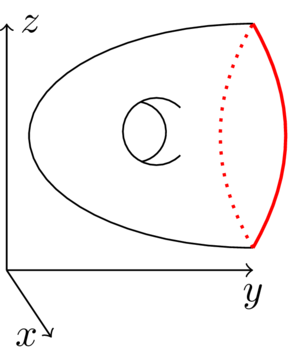
\includegraphics[scale=0.05]{DescendMaps.png}
\caption{Image for Exercise 7}
\end{figure}

\section{Homotopy}

In this section, we will introduce the concept of Homotopy and Homotopy equivalence. Homotopy. Homotopy equivalence is weaker than topological equivalence, but even if it is a weaker concept \emph{homotopy} ``preserve'' some characteristics of the spaces. For example, when we shrink a ball into a point we are making a homotopy, and this shrinking process cannot be a homeomorphism. The relevance of homotopy is that it preserves some form of connectivity, for example, connected components, holes, or voids. A coffee mug is \emph{homotopic} to a circle because they have a hole, but it cannot be to a point or a ball.

\begin{definition}
Let $f: X\to Y$ and $g: X\to Y$ two continuous functions. A \emph{homotopy} is a map $$H: X\times[0,1]\to Y$$ such that 
\begin{enumerate}
\item $H(\cdot, 0)=f,$
\item $H(\cdot,1)=g.$
\end{enumerate}

Two continuous functions are \emph{homotopic} if there exists a homotopy connecting them.
\end{definition} 

\begin{example}
Consider the functions $f: \mathbb{B}^n\to \mathbb{R}^n$ the identity, and $g: \mathbb{B}^n\to\mathbb{R}^n$ that sends everything to the vector $0\in\mathbb{R}^n.$ The maps $f$ and $g$ are homotopic, consider the homotopy $H: \mathbb{B}^3\times[0,1]\to \mathbb{R}^3$ given by $$H(x,t)=(1-t)x.$$ Note that the function $H(\cdot,0)=f$ and $H(\cdot,1)=g.$ 

Therefore, every ball in $\mathbb{R}^n$ is homotopic to a point.
\end{example}

\begin{example}
Consider the functions $f:\mathbb{R}^n\to\mathbb{R}^n$ the identity, and $g:\mathbb{R}^n\to\mathbb{R}^n$ that sends everything to the vector $0\in\mathbb{R}^n.$ The maps $f$ and $g$ are homotopic. The same homotopy of the previous example works. 

In the case that a space $X$ is homotopic to a point, we said that $X$ is \emph{contractible}.
\end{example}

\begin{example}
Consider the functions $f: \mathbb{R}^2 \setminus\{0\} \to \mathbb{R}^2$ the identity, and $g: \mathbb{R}^2\setminus\{0\}\to\mathbb{R}^2$ given by: $g(x)=\frac{x}{||x||}$. The maps $f$ and $g$ are homotopic. Consider the function $H:\mathbb{R}^2\setminus\{0\} \times [0,1]$ given by $$H(x,t)=(1-t)x+tg(x).$$

This example implies that the punctured 2-plane is homotopic to the circle.
\end{example}


 \begin{definition}
 Two topological spaces $X$ and $Y$ are \emph{homotopy equivalent} if there exist maps $g:X\to Y$ and $h:Y\to X$ such that $h\circ g$ is homotopic to the identity $\iota_Y:Y\to Y$ and $g\circ h$ is homotopic to the identity $\iota_X:X\to X.$
 \end{definition}
 
 \begin{example}
We say that the open ball $\mathbb{B}^2\subset \mathbb{R}^2$ is homotopy equivalent to a point. Take $p\in\mathbb{B}^2$ be any point, and consider the maps $h: \mathbb{B}^2\to \{p\}$ the map that sends everything to $p$ and $g: \{p\}\to\mathbb{B}^2$ the map such that $g(p)=q\in\mathbb{B}^2$ where $q$ is any point. 

Note that $h\circ g$ is trivially the identity map, therefore they are homotopic. On the other hand, $g\circ h: \mathbb{B}^2\to\mathbb{B}^2$ is the map that sends the whole $\mathbb{B}^2$ to $q(=g(p)),$ which is homotopic to the identity using the map $$H(x,t)=(1-t)q+tx.$$

Therefore, $\mathbb{B}^2$ and $q$ are homotopy equivalent.
 \end{example}
 
 A more intuitive notion of homotopy equivalent spaces can be derived from the definition of a \emph{deformation retract}, naively speaking there exists a deformation retract between two spaces if they can be seen inside a third space $X$ and they can be deformed from one space into the other.
 
 
  \begin{definition}
  Let $X$ be a topological space, and $U\subset X$ be a subspace. A \emph{retraction} $r$ of $X$ to $U$ is a map $r:X\to U$ such that $r(x)=x$ for every $x\in U.$
  
 The space $U$ is a \emph{deformation retract} of $X$ if the identity map can be continuously deformed to a retraction with no motions of the points already in $U.$
  \end{definition}
  
  In the previous example, note that a point is a deformation retract of an open ball.
 
 \begin{remark}
 If $U$ is a deformation retract of $X,$ then $X$ and $U$ are homotopy equivalent.
 \end{remark}
 
 Homotopy equivalence depends on the space that we are considering the subsets that we want to be homotopic. For example, $\mathbb{S}^1$ is not homotopic equivalent to a point in $\mathbb{S}^1.$ This follows from the fact that if we want a deformation-retract in $\mathbb{S}^1$ it is mandatory to break the continuity of $\mathbb{S}^1$ (break it into pieces).  But, $\mathbb{S}^1$ is homotopic to a point if $\mathbb{S}^1$ is a subset of $\mathbb{S}^2.$
 
 Now that we learned about homotopy equivalence, we can assure that $p$ and $a$ are homotopic to $o.$ And that $l$ and $p$ are not homotopic to each other.
 
 
%\chapter{Second Chapter}
%
%\appendix % From here onwards, chapters are numbered with letters, as is the appendix convention
%
%\pagelayout{wide} % No margins
%\addpart{Appendix}
%\pagelayout{margin} % Restore margins
%
%\chapter{Some more blind-text}


%----------------------------------------------------------------------------------------

\end{document}